\subsection{Problem} \label{subsec:problem}

Self-localization is one of the most fundamental competencies required by an
autonomous robot as the knowledge of its location is an essential precursor to
making decisions about future actions.

One of the simplest forms of self-contained localization is wheel odometry,
based on wheel encoders that are mounted on a robot to track the number of
revolutions each wheel has made. The number of revolutions is integrated into a
dynamic model to determine the robot's current position relative to the
starting point \cite{OdometrySurvey}. But it performs poorly in the presence of
wheel slippage, accumulating position error (drift).

Another form of self-contained localization is visual odometry, which operates
by incrementally estimating the pose of the vehicle through examination of the
changes that motion induces on the images of its onboard cameras
\cite{ScaramuzzaTutorial}. Similarly, laser odometry estimates the ego-motion
of a vehicle by scan-matching of consecutive laser scans. Unlike wheel
odometry, both visual odometry and laser odometry, are not affected by wheel
slip, but they have other drawbacks: visual odometry suffers from poor
illumination and low textured environments; laser might struggle in degenerated
scenes where planar areas are prevalent; both are sensitive to dynamic
environments.

Research that improves the robustness of robot localization can be divided into
two trends: To fuse information from different sensors to overcome their
individual limitations \cite{Valente2019,Vargas2021,Ojeda2006} and to make
better use of the available sensor information using deep learning and other
computationally expensive algorithms \cite{Long2021,DFVO}. Therefore, robot
localization robustness has a price. Whether it is the explicit price of extra
sensors or the implicit cost of extra computational resources.

\begin{figure}[t]
    \centering
    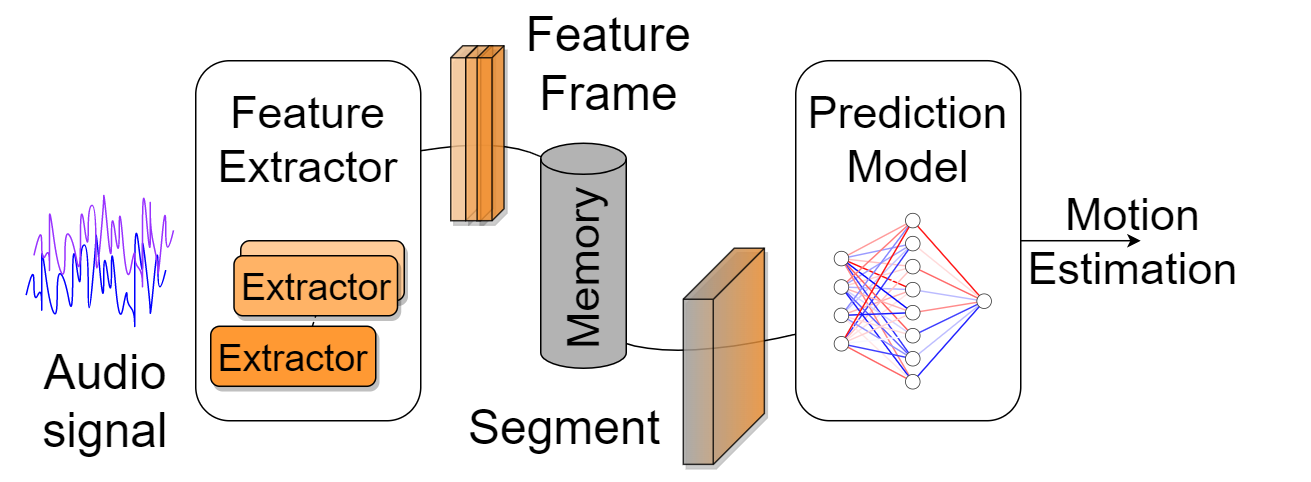
\includegraphics[width=\linewidth]{content/system.drawio.png}
    \caption{Proposed system}
    \label{fig:system}
\end{figure}

